\documentclass{article}
\usepackage{fancyhdr}
\usepackage{amsthm}
\usepackage{etoolbox}
\usepackage{verbatim}
\usepackage{enumerate}
\usepackage{amsmath}
\usepackage{algorithmicx}
\usepackage{algorithm}
\usepackage{algpseudocode}
\usepackage{amssymb}
\usepackage{tikz}
\usepackage{graphicx}
	
\pagestyle{fancy}
\title{Appendix B}
\author{Michelle Bodnar, Andrew Lohr}

\newcounter{curnum}
\setcounter{curnum}{0}

\newtheorem{th1}{Exercise} 
\newcommand{\calH}{\mathcal{H}}
\newcommand{\calX}{\mathcal{X}}
\newcommand{\calA}{\mathcal{A}}
\newcommand{\calY}{\mathcal{Y}}

\begin{document}
\maketitle
\noindent\textbf{Exercise B.1-1}\\
FIrst we consider
\[
A\cap(B\cup C) = (A\cap B)\cup (A \cap C)
\]
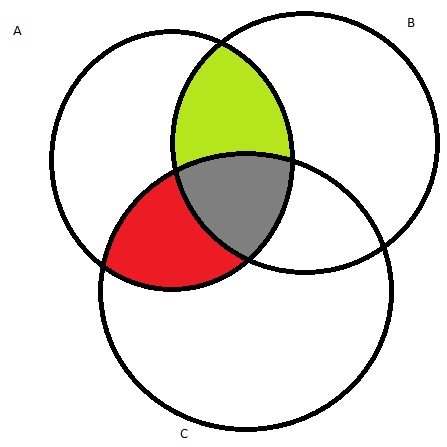
\includegraphics{B(1)}

For the first picture, we can see that the shaded regions are all the regions that are in A and also in either B or C, and so are in the set described on the left hand side. Since the green and gray shaded regions are in both $A$ and $B$, they are in the right hand side, also, the red and gray regions are in $A$ and $C$ and so are also in the right hand side. There aren't any other regions that are either both in A and B or both in A and C, so the shaded regions are the right hand side of the equation as well.


Next we consider
\[
A\cup(B\cap C) = (A\cup B) \cap (A\cup C)
\]
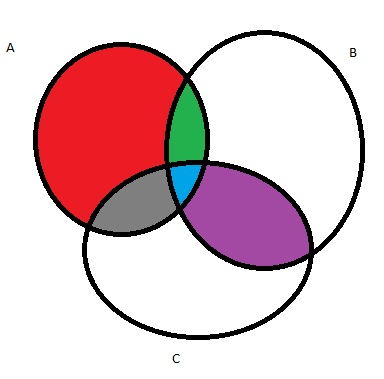
\includegraphics{B(2)}

The ony regions in $B\cap C$ are blue and purple. All the other colored regions are in $A$. So, the shaded regions are exactly the left hand side. To see what is in the right hand side, we see what is both in $A\cup B$ and $A\cap C$. Individually both both contain all of the shaded regions plus one of the white regions. Since the white region contained differs, their intersection is all of the shaded regions.

\noindent\textbf{Exercise B.1-2}\\

We'll proceed by induction.  The base case has already been taken care of for us by B.2.  Suppose that the claim holds for a collection of $n$ sets.  Then we have 
\begin{align*}
\overline{A_1 \cap A_2 \cap \cdots \cap A_n \cap A_{n+1}} &= \overline{(A_1 \cap A_2 \cap \cdots \cap A_n) \cap A_{n+1}} \\
&= \overline{A_1 \cap A_2 \cap \cdots \cap A_n} \cup \overline{A_{n+1}} \\
&= \overline{A_1} \cup \overline{A_2} \cup \cdots \cup \overline{A_n} \cup \overline{A_{n+1}}.
\end{align*}

An identical proof with the roles of intersection and union swapped gives the second result.\\


\noindent\textbf{Exercise B.1-3}\\
%woah I'll come back to it

\noindent\textbf{Exercise B.1-4}\\

Let $f(k) = 2k+1$.  Then $f$ is a bijection from $\mathbb{N}$ to the set of odd natural numbers, so they are countable. \\


\noindent\textbf{Exercise B.1-5}\\
For each of the elements of $S$, some subset of $S$ can either contain that element or not contain that element. If the decision differs for any of the $|S|$ many elements, then you've just created a distinct set. Since we make a decision between two options $|S|$ many times, the total number of possible sets is $2^{|S|}$. It can be thought of as the number of leaves in a complete binary tree of depth $|S|$.\\

\noindent\textbf{Exercise B.1-6}\\

We define an $n$-tuple recursively as $(a_1, a_2, \ldots, a_n) = ((a_1, a_2, \ldots, a_{n-1}), a_n)$.\\


\noindent\textbf{Exercise B.2-1}\\
To see that it is a partial ordering, we need to show it is reflexive, antisymmetric, and transitive. To see that it is reflexive, we need to show $S\subseteq S$. That is, for every $x\in S$, $s\in S$, which is a tautology. To see that it is antisymmetric, we need that if $S_1 \neq S_2$ and $S_1 \subseteq S_2$ then $S_2 \not \subseteq S_1$. Since $S_1\neq S_2$ there is some element that is in one of them but not in the other. Since $S_1 \neq S_2$, we know that that element must be in $S_2$ because if it were in $S_1$ it would be in $S_2$. Since we have an element in $S_2$ not in $S_1$, we have $S_2 \not\subseteq S_1$. Lastly, we show transitivity, suppose $S_1 \subseteq S_2 \subseteq S_3$. This means that any element that is in $S_1$ is in $S_2$. But since it is in $S_2$, it is in $S_3$. Therefore, every element in $S_1$ is in $S_3$, that is $S_2 \subseteq S_3$.


To see that it is not a total order, consider the elements $\{1,2\}$ and $\{2,3\}$. Neither is contained in the other, so there is no proscribed ordering between the two based off of inclusion. If it were a total ordering, we should be able to compare any two elements, which we just showed we couldn't.\\


\noindent\textbf{Exercise B.2-2}\\

For all positive integers $a$ we have $a - a = 0\cdot n$ so the relation is reflexive.  If $a-b = qn$ then $b-a = (-q)n$ so the relation is symmetric.  If $a - b = qn$ and $b-c = pn$ then $a - c = a - b + b - c = (q+p)n$ so the relation is transitive. Thus, equivalence modulo $n$ is an equivalence relation.  This partitions the integers into equivalence classes consisting of numbers which differ by a multiple of $n$.  \\

\noindent\textbf{Exercise B.2-3}\\
\begin{enumerate}[a.]
\item
Consider the set of vertices in some non-complete, non-empty graph where we make two vertices related if they are adjacent or the same vertex.
\item
Consider the vertices in a digraph where we have $aRb$ if there is some possibly empty path from $a$ to $b$. For a concrete example, suppose we have only the set $\{0,1\}$ and the relations $0R0$, $0R1$, and $1R1$.
\item
Consider the relation that makes no two elements related. This satisfies both the symmetric and transitive properties, since both of those require that certain elements are related to conclude that some particular other elements are related.\\

\end{enumerate}

\noindent\textbf{Exercise B.2-4}\\

Suppose that $a R b$.  Since $R$ is an equivalence relation it is symmetric, so $bRa$.  Since $R$ is antisymmetric, $aRb$ and $bRa$ imply that $a = b$.  Thus every equivalence class is a singleton. \\

\noindent\textbf{Exercise B.2-5}\\
Professor Narcissus is full of himself! The relation that makes no two elements related to each other is both symmetric and transitive, but is not reflexive.\\

\noindent\textbf{Exercise B.3-1}\\
\begin{enumerate}[a.]
\item
Since $f$ is injective, for every element in it's range, there is at most one element that maps to it. So, we proceed by induction on the number of elements in the domain of the function. If there is only a single element in the domain, since the function has to map to something, we have that $|B|\ge 1 = |A|$. Suppose that all functions that are on a domain of size $n$ satisfy this relation. Then, look at where that $n+1$st element gets mapped. This point will never be mapped to by any of the other elements of the domain. So, we can think of restricting the function to just the first $n$ elements, and use the inductive assumption to get the desired relation of the two sets.
\item
As a base case, assume that $|B|=1$. Then, since the function is surjective, some element must map to that, so, $|A|\ge 1 = |B|$. Not, suppose it is true for all function with a range of size at most $n$. Then, just look at all the elements that map to the $n+1$st element, there is at least one by surjectivity. This gets us that $|A| \ge 1 + |A'| \ge 1 + |B'| = |B|$.
\end{enumerate}

\noindent\textbf{Exercise B.3-2}\\

When the domain and codomain are $\mathbb{N}$, the function $f(x) = x+1$ is not bijective because 0 is not in the range of $f$.  It is bijective when the domain and codomain are $\mathbb{Z}$. \\


\noindent\textbf{Exercise B.3-3}\\
Define $R^{-1}$ by $a R^{-1} b$ if and only if $b R a$. This clearly swaps the domain and range for the relation, and so, if $R$ was bijective, it is the inverse function. If $R$ was not bijective, then $R^{-1}$ might not even be a function.\\

\noindent\textbf{Exercise B.3-4}\\

It is easiest to see this bijection pictorally.  Imagine drawing out the elements of $\mathbb{Z} \times \mathbb{Z}$ as points in the plane.  Starting from $(0,0)$, move up one unit to $(0,1)$, then right one unit to $(1,1)$, down 2 units through $(1,0)$ to $(1,-1)$, then left, and so on, continuing in a spiraling fashion, hitting each point exactly once, not skipping any as you move outwards.  If point $(i,j)$ is the $k^{th}$ point which is hit, then let $f(i,j) = (-1)^k\lceil k/2 \rceil$.  This gives a bijection from $\mathbb{Z} \times \mathbb{Z}$ to $\mathbb{Z}$, which implies that $f$ has an inverse $g$.  The function $g$ is the desired bijection. \\

\noindent\textbf{Exercise B.4-1}\\
Let $f(u,v)$ be equal to 1 if $u$ shook hands with $v$. Then, $\sum_{v\in V} degree(v) = \sum_{v\in V} \sum_{u\in V} f(v,u)$ then, since handshaking is symmetric, we are counting both when $u$ shakes $v$ hand and when $v$ shakes $u$'s hand. So, this sum is $\sum_{e\in E} 2 = 2|E|$.\\

\noindent\textbf{Exercise B.4-2}\\

Suppose that $u = v_0, v_1, \ldots, v_k = v$ is a path $p$ from $u$ to $v$.  If it is not simple, then it contains a cycle, so there exist $i$ and $j$ such that $v_i = v_j$.  Let $p'$ be the path on vertices $v_0, v_1, \ldots, v_{i-1}, v_j, \ldots, v_k$.  This is a path from $u$ to $v$ which contains at least one fewer cycles than before.  We can continue this process until the path contains no cycles. Similarly, suppose a directed graph contains a cycle $v_0, v_1, \ldots, v_k$.  If it is not simple, then there exist $i$ and $j \neq k$ such that $v_i = v_j$.  Remove the vertices $v_i, v_{i+1}, \ldots, v_{j-1}$ from the cycle to obtain a cycle with at least one fewer duplicate vertices.  Continuing with this process will eventually produce a cycle with no repeated vertices except the first and last, so it will be simple. \\


\noindent\textbf{Exercise B.4-3}\\
We proceed by induction on the number of vertices. If there is a single vertex, then the inequality trivially holds since the left hand side is the size of a set and the right hand side is zero. For the inductive case, pick one vertex in particular. We know that that vertex must have at least one edge to the rest of the vertices because the graph is connected. So, when we take the induced subgraph on the rest of the vertices, we are decreasing the number of edges by at least one. So, $|E| \ge 1+ |E'| \ge 1+ |V'| -1 = |V| -1$.\\

\noindent\textbf{Exercise B.4-4}\\

Every graph is reachable from itself by the empty path so the relation is reflexive.  If $v$ is reachable from $u$ then there exists a path $u = v_0, v_1, \ldots, v_k = v$.  Thus, $v_k, v_{k-1}, \ldots, v_0$ is a path from $v$ to $u$, so $u$ is reachable from $v$ and the relation is symmetric.  If $v$ is reachable from $u$ and $w$ is reachable from $v$ then by concatenation of paths, $w$ is reachable from $u$, so the relation is transitive.  Therefore the ``is reachable from'' relation is an equivalence relation. \\


\noindent\textbf{Exercise B.4-5}\\
The undirected version of the graph in B.2(a) is on the same vertex set, but has $E =\{(1,2),(2,4),(2,5),(4,1),(4,5),(6,3)\}$. That is, we threw out the antisymmetric edge, and the self edge. There is also a difference in that now the edges should be viewed as unordered unlike before.

The directed version of B.2(b) looks the same, except it has arrows drawn in. One from 2 to 1, one from 1 to 5, one from 2 to 5, and one from 3 to 6.\\

\noindent\textbf{Exercise B.4-6}\\

We create a bipartite graph as follows:  Let $V_1$ be the set of vertices of the hypergraph and $V_2$ be the set of hyperedges.  For each hyperedge $e = \{v_1, v_2, \ldots, v_k\} \in V_2$, draw edges $(e,v_i)$ for $1 \leq i \leq k$.  \\


\noindent\textbf{Exercise B.5-1}\\
There are three such rooted trees:

\begin{tikzpicture}[level/.style={sibling distance=50mm/#1}]
\node [circle,draw] (4){x}
  child {
  node [circle,draw] (2) {y}
  }
  child {
  node [circle,draw] (3) {z}    
  }
  ;
\end{tikzpicture}
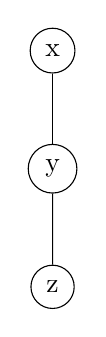
\begin{tikzpicture}[level/.style={sibling distance=50mm/#1}]
\node [circle,draw] (x){x}
  child {
  node [circle,draw] (y) {y}
  child {
  node [circle,draw] (z) {z}    
  }
  }
  ;
\end{tikzpicture}
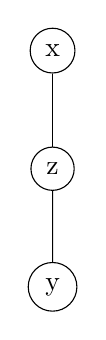
\begin{tikzpicture}[level/.style={sibling distance=50mm/#1}]
\node [circle,draw] (x){x}
  child {
  node [circle,draw] (z) {z}
  child {
  node [circle,draw] (y) {y}    
  }
  }
  ;
\end{tikzpicture}

The ordered trees are those listed above, in addition to the tree

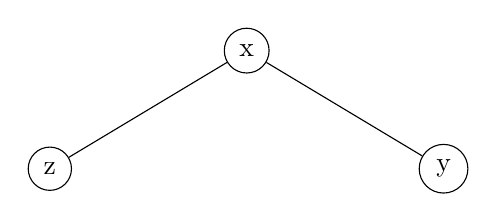
\begin{tikzpicture}[level/.style={sibling distance=50mm/#1}]
\node [circle,draw] (4){x}
  child {
  node [circle,draw] (2) {z}
  }
  child {
  node [circle,draw] (3) {y}    
  }
  ;
\end{tikzpicture}

The Binary trees are all ten of the following:

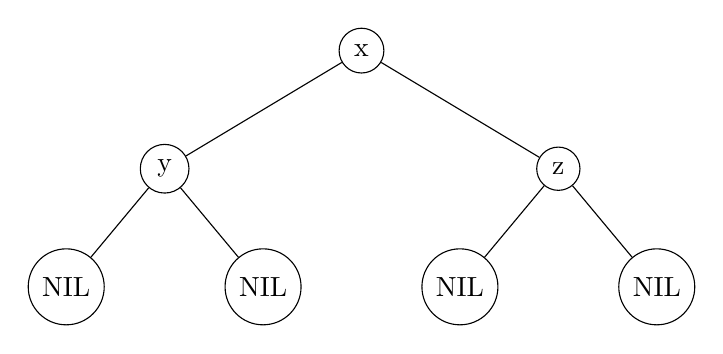
\begin{tikzpicture}[level/.style={sibling distance=50mm/#1}]
\node [circle,draw] (4){x}
  child {
  node [circle,draw] (2) {y}
  child{
  node [circle,draw] (10) {NIL}
  }
  child{
  node [circle,draw] (11) {NIL}
  }
  }
  child {
  node [circle,draw] (3) {z}    
    child{
  node [circle,draw] (12) {NIL}
  }
  child{
  node [circle,draw] (13) {NIL}
  }
  }
  ;
\end{tikzpicture}

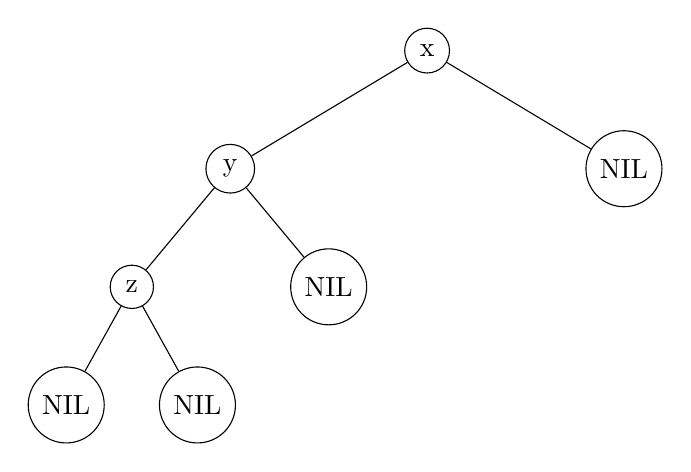
\begin{tikzpicture}[level/.style={sibling distance=50mm/#1}]
\node [circle,draw] (x){x}
    child {
  node [circle,draw] (y) {y}
  child {
  node [circle,draw] (z) {z} 
    child{
  node [circle,draw] (10) {NIL}
  }
  child{
  node [circle,draw] (11) {NIL}
  }
  }
    child{
  node [circle,draw] (12) {NIL}
  }
  }
      child{
  node [circle,draw] (12) {NIL}
  }

  ;
\end{tikzpicture}

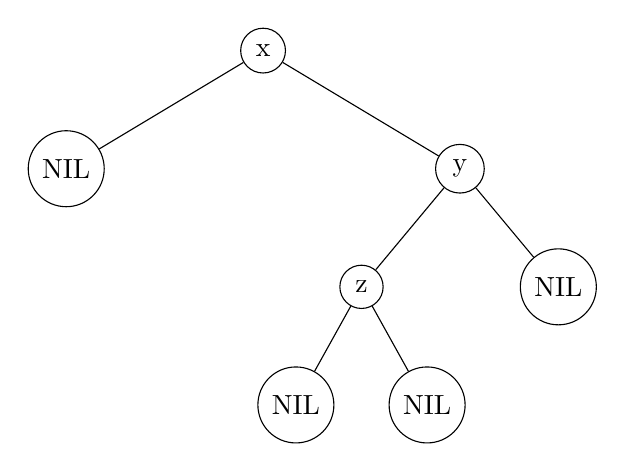
\begin{tikzpicture}[level/.style={sibling distance=50mm/#1}]
\node [circle,draw] (x){x}
    child{
  node [circle,draw] (12) {NIL}
  }
    child {
    node [circle,draw] (y) {y}
  child {
  node [circle,draw] (z) {z} 
    child{
  node [circle,draw] (10) {NIL}
  }
  child{
  node [circle,draw] (11) {NIL}
  }
  }
      child{
  node [circle,draw] (13) {NIL}
  }
  }
  ;
\end{tikzpicture}

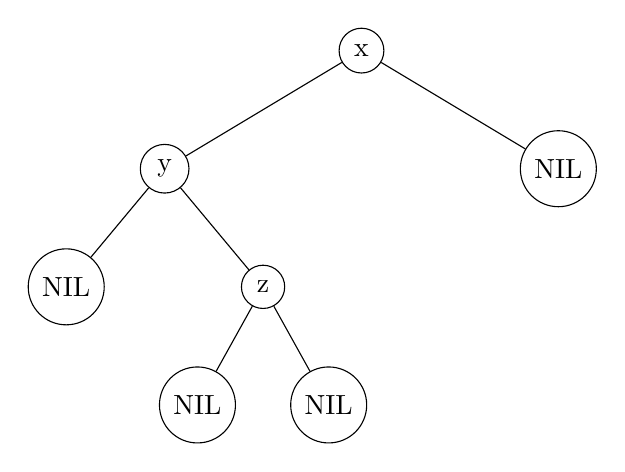
\begin{tikzpicture}[level/.style={sibling distance=50mm/#1}]
\node [circle,draw] (x){x}
    child {
  node [circle,draw] (y) {y}
    child{
  node [circle,draw] (12) {NIL}
  }
    child {
  node [circle,draw] (z) {z} 
    child{
  node [circle,draw] (10) {NIL}
  }
  child{
  node [circle,draw] (11) {NIL}
  }
  }
  }
      child{
  node [circle,draw] (12) {NIL}
  }  ;
\end{tikzpicture}

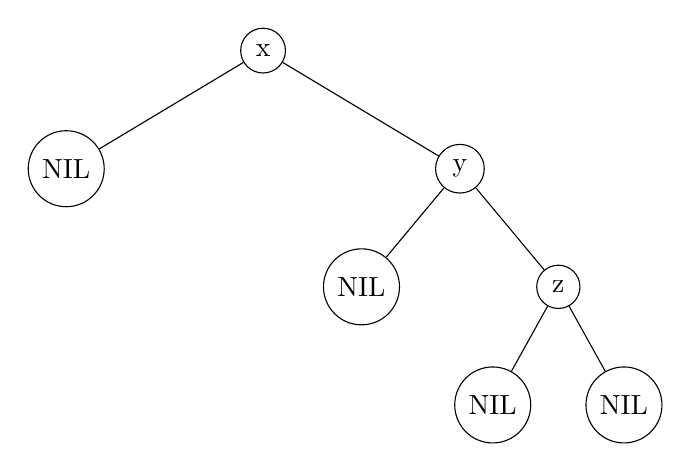
\begin{tikzpicture}[level/.style={sibling distance=50mm/#1}]
\node [circle,draw] (x){x}
    child{
  node [circle,draw] (12) {NIL}
  }
    child {
    node [circle,draw] (y) {y}
      child{
  node [circle,draw] (13) {NIL}
  }
    child {
  node [circle,draw] (z) {z} 
    child{
  node [circle,draw] (10) {NIL}
  }
  child{
  node [circle,draw] (11) {NIL}
  }
  }
  }
  ;
\end{tikzpicture}

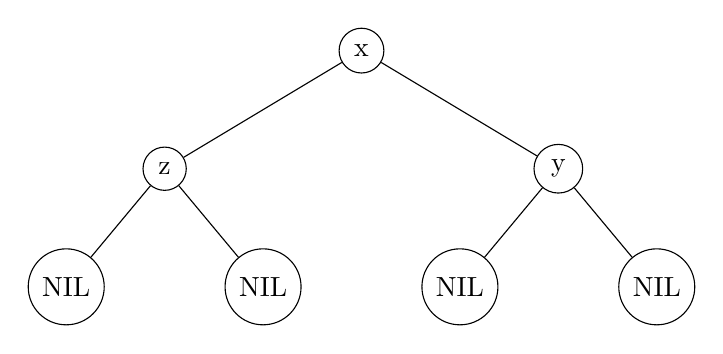
\begin{tikzpicture}[level/.style={sibling distance=50mm/#1}]
\node [circle,draw] (4){x}
  child {
  node [circle,draw] (2) {z}
  child{
  node [circle,draw] (10) {NIL}
  }
  child{
  node [circle,draw] (11) {NIL}
  }
  }
  child {
  node [circle,draw] (3) {y}    
    child{
  node [circle,draw] (12) {NIL}
  }
  child{
  node [circle,draw] (13) {NIL}
  }
  }
  ;
\end{tikzpicture}

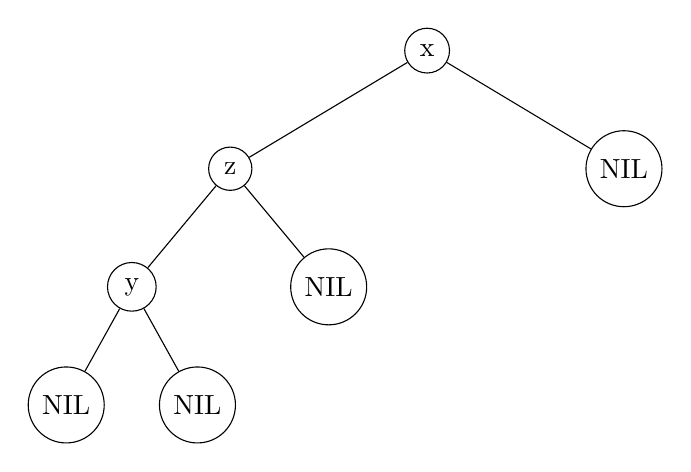
\begin{tikzpicture}[level/.style={sibling distance=50mm/#1}]
\node [circle,draw] (x){x}
    child {
  node [circle,draw] (y) {z}
  child {
  node [circle,draw] (z) {y} 
    child{
  node [circle,draw] (10) {NIL}
  }
  child{
  node [circle,draw] (11) {NIL}
  }
  }
    child{
  node [circle,draw] (12) {NIL}
  }
  }
      child{
  node [circle,draw] (12) {NIL}
  }

  ;
\end{tikzpicture}

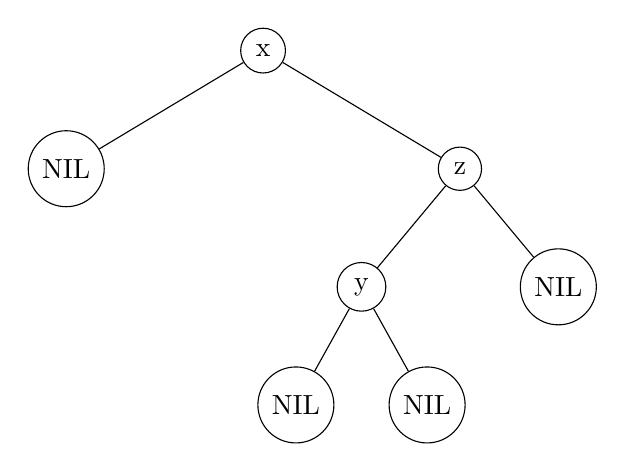
\begin{tikzpicture}[level/.style={sibling distance=50mm/#1}]
\node [circle,draw] (x){x}
    child{
  node [circle,draw] (12) {NIL}
  }
    child {
    node [circle,draw] (y) {z}
  child {
  node [circle,draw] (z) {y} 
    child{
  node [circle,draw] (10) {NIL}
  }
  child{
  node [circle,draw] (11) {NIL}
  }
  }
      child{
  node [circle,draw] (13) {NIL}
  }
  }
  ;
\end{tikzpicture}

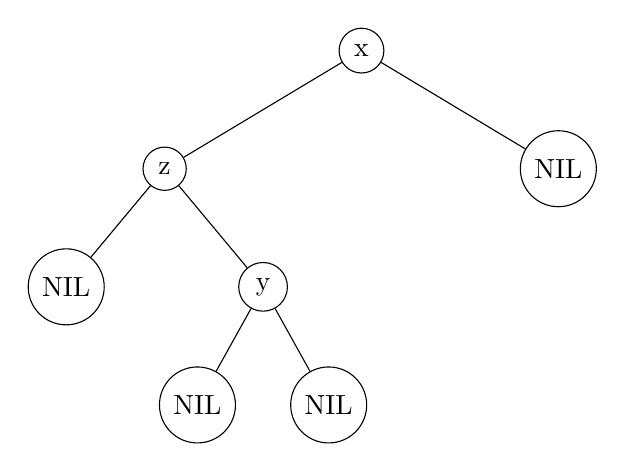
\begin{tikzpicture}[level/.style={sibling distance=50mm/#1}]
\node [circle,draw] (x){x}
    child {
  node [circle,draw] (y) {z}
    child{
  node [circle,draw] (12) {NIL}
  }
    child {
  node [circle,draw] (z) {y} 
    child{
  node [circle,draw] (10) {NIL}
  }
  child{
  node [circle,draw] (11) {NIL}
  }
  }
  }
      child{
  node [circle,draw] (12) {NIL}
  }

  ;
\end{tikzpicture}

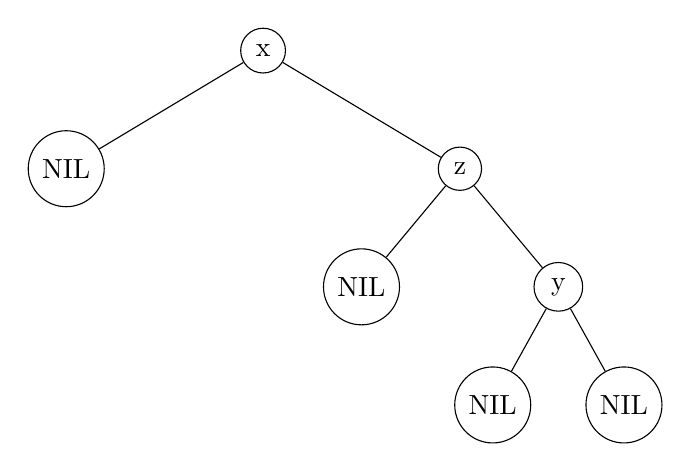
\begin{tikzpicture}[level/.style={sibling distance=50mm/#1}]
\node [circle,draw] (x){x}
    child{
  node [circle,draw] (12) {NIL}
  }
    child {
    node [circle,draw] (y) {z}
      child{
  node [circle,draw] (13) {NIL}
  }
    child {
  node [circle,draw] (z) {y} 
    child{
  node [circle,draw] (10) {NIL}
  }
  child{
  node [circle,draw] (11) {NIL}
  }
  }
  }
  ;
\end{tikzpicture}

\noindent\textbf{Exercise B.5-2}\\

Suppose vertex $u$ is not on the unique path from $v_0$ to $v$ and $v$ is not on the unique path from $v_0$ to $u$.  Then there can't be an edge from $v$ to $u$ or from $u$ to $v$, otherwise we would violate uniqueness.  This implies that in the undirected version of $G$ when we remove the arrows from the edges, there is still a unique path from $v_0$ to every vertex.  This implies that there exists a path between every pair of vertices.  Suppose the path from $u$ to $v$ is not unique. Then there must be a path $p$ from $u$ to $v$ which does not contain $v_0$.  Thus, the unique path from $v_0$ to $v$ differs from the path obtained by going from $v_0$ to $u$, then taking $p$.  This is a contradiction, because the path from $v_0$ to $v$ is unique.  By property 2 of Theorem B.2, $G$ is a free tree.\\


\noindent\textbf{Exercise B.5-3}\\
As a base case, consider the binary tree that consists of a single node. This tree has no degree two nodes and one leaf, so, the number of degree two nodes is one less than the number of leaves. As an inductive step, suppose it is true for all binary trees with at most $n$ degree two nodes. Then, let $G$ be a binary tree with $n+1$ internal nodes. Let $v$ be the first node, possibly the leaf itself, that is the child of a degree two node, and can be obtained by taking the parent pointer from the leaf. Then, consider the tree obtained by removing $v$ and all its children. Doing so removes only one leaf, and it makes the parent of $v$ drop to being degree 2. None of the children of $v$ were degree 2 because otherwise we would of stopped earlier when we were selecting $v$. Since we have decreased the number of degree two nodes and leaves both by 1, we have completed the inductive case, because if $|T'|$ is the modified tree, the number of leaves in $T$ is one more than that in $T'$ which means it is one more than the number of degree 2 nodes in $T'$, which is the number of degree two nodes in $T$.

Since a full binary tree has each internal node with degree two, this result gets us that the number of internal nodes in a full binary tree is one more than the number of leaves.\\

\noindent\textbf{Exercise B.5-4}\\

A tree with 1 node has height at least 0, so the claim holds for $n=1$.  Now suppose the claim holds for $n$.  Let $T$ be a binary tree with $n+1$ nodes.  Select a leaf node and remove it. By our induction hypothesis, the resulting tree has height at least $\lfloor \lg n \rfloor$. If $n+1$ is not a power of 2 then this is equal to $\lfloor \lg(n+1) \rfloor$, so we are done.  Otherwise, choose a leaf of greatest depth to remove.  The resulting tree has height at least $\lfloor \lg n \rfloor$.  If the height in fact achieves that, then the only possible tree is the complete binary tree on $n$ vertices.  Since every internal node has two children, the only place the removed leaf could have come from is from a leaf vertex.  Adding a child to any leaf vertex increases the height of the tree by 1.  Since $\lfloor \lg n\rfloor + 1 \geq \lfloor \lg(n+1) \rfloor$, the claim holds. \\

\noindent\textbf{Exercise B.5-5}\\
We will perform structural induction. For the empty tree that has $n=0$, the equation is obviously satisfied. Now, let $r$ be the root of the tree $T$, and let $T_L$ and $T_R$ be the left and right subtrees respectively. By the inductive hypothesis, we may assume that $e_L = i_L + 2n_L$ and $e_R = i_R + 2 n_R$. Then, since being placed as a child of the root adds one to the depth of each of the nodes in both $T_L$ and $T_R$, we have that $i = i_L + i_R + n_L+n_R$ and 
\begin{align*}
e =& e_L + |leaves(T_L)| + e_R +|leaves(T_R)| \\
=& e_L + e_R + |leaves(T)| \\
=& i_L + 2 n_L + i_R + 2n_R + |leaves(T)| \\
=& i + n_L + n_R + |leaves(T)| \\
=& i + n-1 + |leaves(T)| \\
\end{align*}
 By problem B.5-3, since the tree is full, we know that $|leaves(T)|$ is one more than the number of internal nodes of $T$. So, $e =  i+ 2n$, completing the induction.\\

\noindent\textbf{Exercise B.5-6}\\

We'll proceed by strong induction on the number of nodes in the tree.  When $n=1$, there is a single leaf which has depth 0, so we have $\sum_{x \in L} w(x) = 2^{-0} = 1$.  Now suppose the claim holds for a tree with at most $n$ nodes and let $T$ be a tree on $n+1$ nodes.  If the left or right subtree of $T$ is empty then the induction hypothesis tells us that the subtree on the nonempty side satisfies the inequality with respect to depth in that tree.  Since the depth in the original tree is one greater for each leaf, the claim holds. On the other hand, if $T$ has left and right children, call the subtrees rooted at the children $T_1$ and $T_2$.  By the induction hypothesis, the sums of the weights of their leaves are each less than or equal to 1.  Since the depth of a node in $T$ is one greater than its depth in $T_1$ or $T_2$, the weight of each leaf in $T$ is halved.  Thus, the sum of the weights of the leaves in each subtree is bounded by 1/2, so the total sum of weights of leaves is bounded by 1. \\

\noindent\textbf{Exercise B.5-7}\\
Suppose to a contradiction that there was some binary tree with more than 2 leaves that had no subtree with a number of leaves in the desired range. Since $L>1$, the root is not a leaf. Now, define the sequence $x_0 = root$, $x_{i+1}$ is the larger(more leaves) of the children of $x_i$, until we have reached a root. Now, we consider the number of leaves in the subtree rooted at each $x_i$. For $x_0$ it is $L$, which is too large, and at $x_h$, it is $1$ which is not too large. Now, we keep incrementing from $x_0$ to $x_1$ to $x_2$, and so on until we have some number of leaves that falls in the desired range. If it happens we are done and have contradicted the assumption that this binary tree didn't have such a subtree. Since it doesn't that means there is some step where the number of leaves jumps from more than $2L/3$ to less than $L/3$, Since both of the children of the next $x_i$ were less than $L/3$, their sum cannot be more than $2L/3$, a contradiction.

\noindent\textbf{Problem B-1}\\
\begin{enumerate}[a.]
\item If the tree is unrooted, pick an arbitrary node to be the root. Assign color 0 to all nodes that are at an even height, and assign color 1 to all nodes that are at an odd height. Since the child of any node has height one greater, there will never be two adjacent nodes that have received the same color.
\item We show the following implications in order to get equivalence of all three
\begin{enumerate}
\item[$1\Rightarrow 2$] Since the graph is bipartite, we can partition the vertices into two sets $L$ and $R$ so that there are no edges going between vertices in $L$ and no edges going between vertices in $R$. This means that we can assign color 0 to all vertices in $L$ and color 1 to all vertices in $R$ without having any edges going between two vertices of the same color.
\item[$2\Rightarrow 3$]
Suppose to a contradiction that there was a cycle of odd length, but we did have a valid two coloring. As we go along the cycle, each time we go to the next vertex, the color must change because no two adjacent vertices can have the same color. If we go around the cycle like this though, we have just flipped the color an odd number of times, and have returned back to the original color, a contradiction.
\item[$3\Rightarrow 2$]
If $G$ has no cycles of an odd length, then we can just perform the greedy operation to two color. That is, we pick a vertex, color it arbitrarily, then, for any vertex adjacent to a colored vertex, we color it the opposite color. If this process doesn't end up coloring everything, i.e. the graph is disconnected, we repeat it. Since the only way this process could fail is if there is an odd length cycle, it provides a two coloring, proving that the graph is two colorable.
\item[$2\Rightarrow 1$]
Partition the vertices based on what color they received. Since there are no edges going between the vertices of the same color, there won't be any edges going between vertices that are in the same part in the partition.
\end{enumerate}
\item
Consider the process where we pick an arbitrary uncolored vertex and color it an arbitrary color that is not the color of any of its neighbors. Since a vertex can only have at most $d$ neighbors, and there are $d+1$ colors to choose from, this procedure can always be carried out. Also, since we are maintaining at each step that there are no two adjacent vertices that have been colored the same, we have that the end result of all the coloring is also valid.
\item
Let $V'$ be the set of vertices whose degree is at least $\sqrt{|E|}$. The total number of edges incident to at least one of these vertices is at least $\frac{|V'|\sqrt{|E|}}{2}$ by exercise B.4-1. Since this also has to be bounded by the total number of edges in the graph, we have that $\frac{|V'|\sqrt{|E|}}{2} \le |E|$, which gets us that $|V'| \le 2\sqrt{|E|}$. So, we'll assign all of the vertices in $V'$ their own distinct color. Then, so long as we color the rest of the edges with colors different from those used to color $V'$, the edges between $V'$ and the rest of the vertices won't be important for affecting the validity of the coloring. So, we look at the graph induced on the rest of the vertices. This graph is degree at most $\sqrt{|E|}$ because we already removed all the vertices of high degree. This means that by the previous part, we can color it using at most $\sqrt{|E|} +1$ colors. Putting it together, the total number of colors used to obtain a valid coloring is $2 \sqrt{|E|} + \sqrt{|E} +1 \in O(\sqrt{|E|}) = O(\sqrt{|V|})$.
\end{enumerate}

\noindent\textbf{Problem B-2}\\

\begin{enumerate}[a.]
\item Any undirected graph with at least two vertices contains at least two vertices of the same degree.  Proof: Suppose every vertex has a different degree.  Since the degree of a vertex is bounded between 0 and $n-1$, the degrees of the vertices must be exactly $0, 1, \ldots, n-1$.  However, if some vertex has degree 0 then no vertex can have degree $n-1$.  Thus, some pair of vertices must have the same degree. \\

\item Every undirected graph on 6 vertices contains 3 vertices which are all connected to one another or 3 vertices among which there are no edges.  Proof:  Suppose that we have a graph which doesn't have this property.  We'll show such a graph cannot exist.  If vertex 1 has degree at least 3, then there can be no edges among these vertices connected to 1.  Otherwise there would be a triangle.  However, if there are no edges among these vertices then there are at least 3 among which there are no edges.  Thus vertex 1 must have degree at most 2.  Since there was nothing special about this vertex, the same argument tells us that every vertex must have degree at most 2.  Now consider the graph $G' = (V, E')$ where $E' = \{(u,v) | (u,v) \notin E\}$.  Observe that $G$ has no 3 mutually connected or mutually disconnected vertices if and only if $G'$ does, so the same argument tells us that every vertex of $G'$ has at most degree 2, which implies that ever vertex of $G$ has degree at least 4, a contradiction.\\

\item The vertex set $V$ of any undirected graph can be partitioned into $V = V_1 \sqcup V_2$ such that at least half of the neighbors of each $v \in V_1$ are in $V_2$, and at least half of the neighbors of each $v \in V_2$ are in $V_1$.  Proof: Consider an abritrary partition $V_1 \sqcup V_2$.  For each edge $(u,v)$ where $u \in V_1$ and $v \in V_2$, do the following:  If $u$ and $v$ already have the property that more than half of their neighbors are in the opposite partition, do nothing.  If both $u$ and $v$ fail to have this property, swap which partition $u$ and $v$ are in.  Now suppose just one vertex fails.  Without loss of generality, suppose it is $u$.  If $v$ has at least one more than half its neighbors in $V_1$, simply move $u$ into $V_1$.  Otherwise, swap $u$ and $v$.  Each time we do this for an edge $(u,v)$, the number of edges from $V_1$ to $V_2$ strictly increases.  For an edge $(u,v)$ with $u$ and $v$ in the same partition, if either $u$ or $v$ has more than half its neighbors in its own partition, move it to the other partition.  If both do, just move $u$.  Again, this will strictly increase the number of edges between $V_1$ and $V_2$.  Keep picking edges and repeating this process.  Since the number of edges between $V_1$ and $V_2$ cannot increase indefinitely, this process will eventually stop, and every vertex will have the property that at least half its neighbors are in the opposite partition.\\

\item If every vertex of an undirected graph has degree at least $|V|/2$ then there exists a way to draw the graph where the vertices all lie on a circle, and vertices next to one another on the circle are always connected by an edge. Proof: Let $|V| = n$.  It is easy to check that the claim holds from $n=1, 2, 3$.  We'll proceed by induction on $n$.  Supoose the claim holds for all graphs on $\leq n $ vertices and let $G$ be a graph on $n+1$ vertices such that each vertex has degree at least $(n+1)/2$.  If $n$ is odd, consider the arrangement of the induced subgraph on $n$ vertices.  There must exist some pair of adjacent vertices both of which are connected to the $(n+1)^{st}$ vertex by an edge, so we may insert it there.  If $n$ is even, it could be the case that vertex $n+1$ is connected to every other vertex in the arrangement on $n$ vertices.  In this case, select a pair of vertices which are separated by 2 edges on the circle, both of which are connected to $n+1$.  Replace the vertex $v$ between them by $n+1$.  Excluding vertex $n+1$, its two adjacent vertices (on the circle), and $v$, there are $n-3$ remaining vertices.  Since $n$ is even, $n-3$ is odd.  Since $v$ is connected to at least $(n-3)/2$ of these, there must exist 2 which are adjacent on the circle.  We can safely place $v$ inbetween these to obtain the desired graph. 
\end{enumerate}


\noindent\textbf{Problem B-3}\\
\begin{enumerate}[a.]
\item
Suppose that $n \ge 4$, as all smaller binary trees can be easily enumerated and this fact checked for. Start at the root, let that be $x_0$, then, let $x_{i+1}$ be the larger child of $x_i$, or it's only child if there is just one. Eventually this process will stop once it has reached a root. Let $s(v)$ be the size of the subtree rooted at $v$. Since we always pick the larger of the two subtrees, we have that $s(x_i) \le 2s(x_{i+1}) +1$. So, if we have that $s(x_{i+1}) \le n/4$, then, we have that $s(x_i) \le 2 n/4 +1 \le 3n/4$. Since eventually this sequence goes to 1, which is below the range, and it starts at n, which is above, we must have that at some point it dips below, the parent of this node is the one that we need to snip off of the original tree to get the desired size subtree.

\item
Take a binary tree on four vertices as follows:

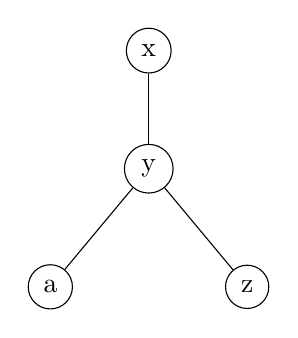
\begin{tikzpicture}[level/.style={sibling distance=50mm/#1}]
\node [circle,draw] (x){x}
    child {
  node [circle,draw] (y) {y}
    child{
  node [circle,draw] (12) {a}
  }
    child {
  node [circle,draw] (z) {z} 
  }
  }
  ;
\end{tikzpicture}

Where it is unimportant whether y is the left or right child of $x$. Then, any cut that is made of the three edges in the graph results in there being one set of vertices of size 3 that are connected and one vertex that is all by its lonesome self. This means that the larger of the two sets the vertices is partitioned into has size $3 = (3/4) \cdot n$. 

\item
We will make a single cut to the original tree to take off a piece that is less than or equal to $\lfloor\frac{n}{2}\rfloor$. As in part a, we let $x_0$ be the root, and let $x_{i+1}$ be the larger child of $x_i$. We show that the size of the subtree rooted at $x_i$, say $s(x_i)$ can old drop by at most a factor of 3. To do this, we use the fact that $s(x_i) \le 2s(x_{i+1})+1$. So, if $s(x_{i+1}) \le \frac{s(x_{i})}{3}$, then,
\begin{align*}
s(x_i) &\le 2 s(x_{i+1}) +1 \le \frac{2s(x_i)}{3} +1\\
\frac{s(x_i)}{3} &\le 1\\
s(x_i) &\le 3 
\end{align*}
However, for there to even be a $x_{i+1}$, it must have size at least one, so, even then, we have that has dropped by at most a factor of 3.

This means that we can always select a tree that is less than a fact of three below $\lfloor \frac{n}{2}\rfloor$. So, what we do is cut off that subtree, decrease the amount we are trying to cut off by that amount, and then continue. Each cut doing this procedure must decrease the most significant digit of the ternary representation of the amount need to be cut off by 1. This means that it needs at most $2 \log_3(n)$ many cuts, but this is $O(\lg(n))$, so, we are done.
\end{enumerate}

\end{document}